\documentclass{utap}

\usepackage{wrapfig}
\usepackage{xepersian}

\graphicspath{{./img/}}

\title{تمرین شماره‌ی ۵}
\author{
	\href{mailto:bardia.eghbali@gmail.com??subject=[AP\%20S98\%20A5]\%20}{بردیا اقبالی},
	\href{mailto:seyedahmadpourihosseini@gmail.com?subject=[AP\%20S98\%20A5]\%20}{احمد پوری‌حسینی},
	\href{mailto:ahhabibvand@gmail.com?subject=[AP\%20S98\%20A5]\%20}{امیرحسین حبیب‌وند},
	\href{mailto:farzadhabibii98@gmail.com?subject=[AP\%20S98\%20A5]\%20}{فرزاد حبیبی}
}
\course{برنامه‌سازی پیشرفته}
\lecturer{رامتین خسروی}
\deadline{جمعه ۶ اردیبهشت ۱۳۹۸، ساعت ۲۳:۵۵}

\begin{document}
	\maketitle

	\section*{ سوپر ماریو }
مقدمه

برای مشاهده‌ی یک پیاده‌سازی کامل از بازی سوپر ماریو می‌توانید به \href{https://supermariobros.io/}{اینجا} 	مراجعه کنید.
	\pagebreak

	\section{پیش‌تمرین}

در این پیش‌تمرین برنامه‌ای ساده را با کتاب‌خانۀ RSDL پیاده‌سازی می‌کنید تا بیشتر با آن آشنا شوید.


با کمک دستور draw\_img و استفاده از آرگومان src آن، می توانید تکه ای از یک تصویر را روی صفحه رسم کنید. در پوشه warmup تصویری از یک جدول 3x3 است که با اعداد 1 تا 9 پر شده. با استفاده از روش بالا برنامه ای بنویسید که به صورت تصادفی این جدول را به هم ریخته و روی صفحه رسم کند.

حالا می خواهیم با زدن دکمه R ترتیب خانه‌ها تغییر کند. برای این کار داخل یک حلقه با استفاده از تابع poll\_for\_event و get\_pressed\_key چک کنید که آیا دکمه‌ی R زده شده است یا نه. سپس مستطیل‌ها را دوباره محاسبه کنید و صفحه را بروزرسانی کنید.

تصویر زیر پنجره‌ی این برنامه را نشان می‌دهد.
	\begin{center}
		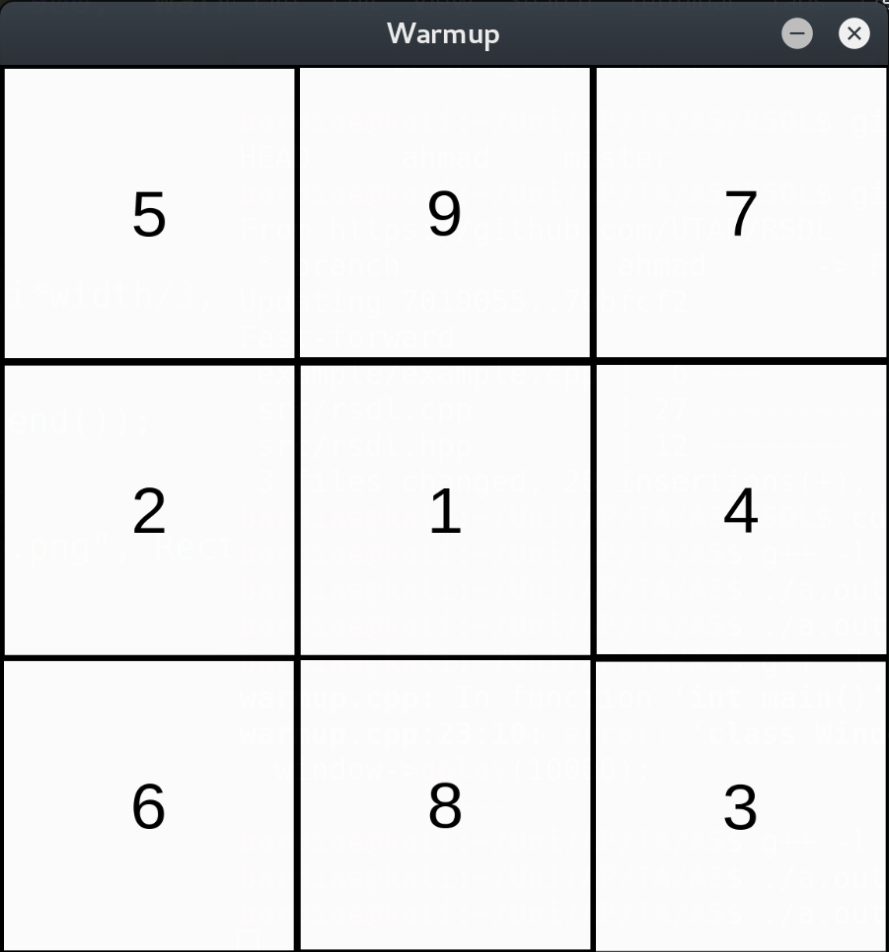
\includegraphics[width=8cm]{warmup.png}
	\end{center}
توجه کنید که این بخش برای آشنایی بیشتر شما با RSDL است و نیازی به تحویل آن نیست.
	\pagebreak

	\section{تمرین}
در این تمرین از شما انتظار می‌رود موارد زیر را پیاده‌سازی کنید و نکات گفته شده را رعایت کنید. تمرین از چند بخش مختلف تشکیل شده است که در ادامه به توضیح هر یک می‌پردازیم.

	\subsection{نقشه}
نقشه‌ی بازی به صورت یک جدول ۲ بعدی از کاراکترها به شما داده می‌شود. هر کاراکتر نشان‌دهنده‌ی محتوای یک خانه \LTRfootnote{tile} از نقشه‌ی بازی است. جدول زیر معنی هر کاراکتر را مشخص می‌کند.
	\begin{table}[H]
		\centering
		\begin{tabular}{ccc}
			\hline
			عنوان & کاراکتر معادل & تصویر\\
			\hline
			آجر‌ساده & b & تصویر\\
			\hline
			آجر شگفت انگیز دارای سکه & ? & تصویر\\
			\hline
			آجر شگفت انگیز دارای قارچ & m & تصویر\\
			\hline
			آجر شگفت انگیز دارای قارچ سلامتی & h & تصویر\\
			\hline
			بلوک معمولی & @ & تصویر\\
			\hline
			بلوک زمینی & \# & تصویر\\
			\hline
			ماریو & M & تصویر\\
			\hline
			گومبا کوچولو & l & تصویر\\
			\hline
			کوپا تروپا & k & تصویر\\
			\hline
			لوله  & | & تصویر\\
			\hline
			پرچم & f & تصویر\\
			\hline
		\end{tabular}
	\end{table}
عکس های مربوطه را می‌توانید در پوشه‌ی assets پیدا کنید. همچنین عکس پس‌زمینه‌ نیز داخل همین پوشه قرار دارد که باید پشت تمامی تصاویر دیگر رسم شود.

توجه کنید که پیاده‌سازی شما نباید به یک نقشه‌ی خاص برای بازی وابسته باشد، و باید بتواند با هر نقشه‌ی دلخواهی که مطابق فرمت گفته شده باشد، \textbf{بدون نیاز} به کامپایل مجدد، اجرا شود. به این  منظور برنامه‌ی شما باید آدرس نقشه‌ی مرحله‌ی مورد نظر را از خط‌فرمان\LTRfootnote{command line} دریافت کند. در هنگام تحویل پروژه، برنامه‌ی شما با یک نقشه‌ی جدید که قبلا ندیده‌اید تست خواهد شد.

	\subsection{دوربین}
همان‌طور که  احتمالا متوجه شده‌اید، نقشه‌ی بازی از ناحیه‌ای که دوربین بازی می‌تواند نشان دهد، بسیار بزرگ‌تر است. در نتیجه نیاز است که با حرکت ماریو به سمت جلو، دوربین نیز او را دنبال بکند. یعنی وقتی ماریو به لبه‌ی راستی صفحه نزدیک می‌شود باید دوربین نیز کمی به راست برود تا ماریو از صفحه خارج نشود. اینکه مرز این جابه‌جایی دوربین چقدر باشد به عهده‌ی خود شما است و صرفا طبیعی بودن آن کافیست.

توجه کنید که ماریو هیچ گاه نباید بتواند از لبه‌ی سمت چپ صفحه خارج شود، در نتیجه دوربین هیچ‌گاه نیاز نیست به سمت چپ حرکت کند.

نگران خارج شدن ماریو در راستای عمودی صفحه نباشید، نقشه‌هایی که در اختیار شما قرار می‌گیرند نیازی به جابه‌جایی دوربین در این راستا نخواهند داشت.

همچنین در نظر داشته باشید که عکس پس‌زمینه بازی هم باید حرکت کند. در واقع در هر لحظه باید بخشی از آن را نمایش دهید و با جابه‌جایی دوربین بخش بعدی عکس را به کاربر نمایش دهید تا حس حرکت در کاربر القا شود.
	\subsection{حرکات}
		\subsubsection{ماریو}
حرکات ماریو در این بازی بسیار ساده هستند. ماریو باید با فشار دادن کلید‌های d و a به ترتیب به سمت راست و چپ حرکت کند، وهم‌چنین با فشار دادن کلید w بپرد. توجه بکنید که ساختار جدول-مانند نقشه، فقط به منظور راحتی ذخیره کردن و خواندن نقشه است، و حرکت‌های داخل بازی ریزدانه‌تر از خانه‌های نقشه، و در مقیاس پیکسل هستند. حرکت ماریو در راستای محور y ها همواره از فرمول های حرکت با شتاب ثابت پیروی می‌کند، یعنی:
	\begin{center}
		$\Delta y = v_y \Delta t$

		$\Delta v_y = g \Delta t$
	\end{center}
و حرکت در راستای محور x ها نیز از فرمول حرکت با سرعت ثابت تبعیت می‌کند، یعنی:
	\begin{center}
		$\Delta x = v_x \Delta t$
	\end{center}
که در این فرمول‌ها $v_y$ و $v_x$ به ترتیب سرعت در راستای y و سرعت در راستای x بوده، و $g$ شتاب گرانشی است. (معمولا ما فرمول‌های سقوط آزاد را به شکل
$y = \frac{-1}{2}gt^2 + v0_y t$
می‌بینیم، که برای محسابه‌ی مستقیم جابه‌جایی آسان‌تر هستند، ولی استفاده از فرمول‌های بالا برای پیاده‌سازی کامپیوتری راحت تر می‌باشند.)

با توجه به این فرمول‌ها در واقع فشار دادن دکمه‌ی پرش باعث ایجاد یک سرعت اولیه در راستای‌ y می‌شود. مشخص کردن مقدار دقیق ثابت $g$ و مقدار $v_x$ به عهده‌ی خود شما است، و لازم و کافی است که این مقادیر طوری انتخاب شوند که حرکت ماریو طبیعی بوده و مشابه لینک داده شده در ابتدای تمرین باشد. طبیعتا این فرمول‌ها فقط در حالتی برقرار هستند که مانعی در سر راه ماریو وجود نداشته باشد، چرا که در این صورت حرکت ماریو در آن راستا متوقف می‌شود.
		\subsubsection{دشمنان}
در این بازی از شما خواسته می‌شود که دو نوع دشمن را پیاده‌سازی کنید، توضیحات این دو نوع در بخش دشمنان آمده است. اما همه‌ی دشمنان ویژگی‌های مشترکی در حرکت خود دارند که در این بخش به آن‌ها می‌پردازیم.

دشمنان در این بازی در ابتدا در مکان اولیه‌ی خود ساکن هستند، و در همین وضعیت می‌مانند تا وقتی که وارد کادر دوربین بازی شوند. پس از ورود به کادر دوربین دشمنان شروع به حرکت به سمت چپ کرده، و تا وقتی مانعی جلو‌ی آن ها نباشد به حرکت خود ادامه می‌دهند. هر وقت که دشمنی به مانعی در مسیر حرکت خود برخورد کند، جهت حرکت خود را تغییر می‌دهد (از راست به چپ، یا از چپ به راست).

برخلاف بازی اصلی، در این تمرین دشمنان برای هم مانع نیستند، یعنی دشمنان می‌توانند از یکدیگر عبور کنند. تنظیم سرعت حرکت دشمنان نیز، مانند ماریو، بر عهده‌ی خود شما است، و کافی است که حرکت و سرعت دشمنان طبیعی و مشابه لینک داده شده در ابتدای تمرین باشد.

از شما انتظار می‌رود با استفاده از عکس‌های داده شده، حس اینکه ماریو و دشمنان در حرکت پاهای خود را تکان می‌دهند را به‌وجود بیاورید.

	\subsection{موانع}
در این بازی سه مانع مختلف وجود دارد، که جلوی ورود ماریو را به خانه‌ای که داخل آن هستند میگیرند:
	\begin{itemize}
		\item
\textbf{بلوک‌ها:}
ساده‌ترین موانع موجود در بازی. اندازه‌ی آن‌ها همیشه به اندازه‌ی یک خانه‌ از نقشه‌ی بازی است. بلوک ها خود دو نوع معمولی و زمینی دارند، که تفاوت آن ها فقط در ظاهرشان است. این تفاوت را می‌توانید در جدول بخش نقشه‌ی بازی مشاهده کنید.
		\item
\textbf{لوله‌ها:}
این موانع کمی از بلوک‌ها پیچیده‌تر هستند. ارتفاع این موانع می‌تواند تا حد دلخواه زیاد باشد، ولی عرض آن ها همواره برابر دو خانه‌ از نقشه است. همچنین این موانع همواره عمودی هستند. شما باید از عکس‌های داده شده استفاده کنید، تا ظاهر لوله را مشابه لینک داده شده در ابندای پروژه بسازید.
		\item
\textbf{آجرها:}
این موانع، بر خلاف دو مانع قبلی که روی زمین هستند، همواره از زمین فاصله دارند. وقتی ماریو از پایین به آجری ضربه می‌زند، آجر کمی به بالا پرتاب می‌شود و اگر دشمنی روی آن‌ باشد، آن را از بین می‌برد، سپس به موقعیت اول خود برمی‌گردد. آجرها ۲ نوع مختلف به شرح زیر دارند:
		\begin{itemize}
			\item
\textbf{معمولی:‌}
این آجرها از آجر‌های شگفت‌انگیز ضعیف‌ترند. به این معنا که به هنگام ضربه زدن ماریو به آن ها از پایین، اگر ماریو بزرگ باشد، می‌شکنند. این آجر ها هیچ‌وقت محتوایی ندارند.
			\item
\textbf{شگفت انگیز:}
این آجرها که با علامت سوال مشخص شده‌اند، محکم هستند، و هیچ‌گاه نمی‌شکنند. اما وقتی ماریو از پایین به آن ها ضربه میزند، محتوای آن‌ها بیرون می‌آید. پس از بیرون آمدن محتوایشان،‌ این آجر‌ها تغییر شکل داده و علامت سوالشان از بین می‌رود.
		\end{itemize}
	\end{itemize}

	\subsection{دشمنان}
در این بازی دو نوع دشمن وجود دارد، که قبل از اینکه به ویژگی‌های هر یک بپردازیم، ابتدا ویژگی‌های مشترک دشمنان را بررسی میکنیم.
همه‌ي دشمنان، همانطور که در بخش حرکت توضیح داده شد، وقتی که وارد کادر بازی می‌شوند، به طور خودکار شروع به حرکت به سمت چپ می‌کنند.
وقتی ماریو به یکی از دشمنان برخورد کند، اگر این برخورد از بالای سر دشمن باشد، آن دشمن آسیب می‌بیند، ولی ماریو آسیبی نمی‌بیند و در عوض فقط کمی به بالا پرتاب می‌شود (مهم است که این به بالا پرتاب شدن را پیاده سازی کنید). اما اگر این برخورد از جهتی دیگر باشد، ماریو یک جان خود را از دست داده، و به ابتدای مرحله برمی‌گردد. دشمنان این بازی عبارتند از:
	\begin{itemize}
		\item
\textbf{گومبا کوچولو\LTRfootnote{Little Gomba}:}
گومباها ساده‌ترین دشمنان در این بازی هستند. این دشمنان به محض برخورد با ماریو از بالای سرشان از بین می‌روند. البته قبل از اینکه کامل از بازی حذف شوند، برای چند ثانیه بدن مرده‌ی آن‌ها روی زمین باقی می‌ماند، و پس از مدت کوتاهی دیگر اثری از آن‌ها در بازی باقی نمی‌ماند.
		\item
\textbf{کوپا تروپا\LTRfootnote{Koopa Troopa}:}
این دشمنان کمی پیچیده‌ترند. وقتی ماریو از بالا به کوپا تروپا برخورد می‌کند کوپاتروپا به صورت برعکس روی زمین قرار می‌گیرد و دیگر حرکت نخواهد کرد. با برخورد بعدی ماریو با کوپا‌تروپا از سمت بالا، این موجود در جهت مناسب پرتاب می‌شود. در این حالت، کوپا تروپا با هر چیزی که برخورد کند، آن را بلافاصله می‌کشد (کوپاتروپاهای دیگر نیز بلافاصله می‌میرند و برعکس روی زمین نمی‌افتند)، و مشابه تمامی حرکت‌های دیگر، وقتی تروپا در این حالت به مانعی برخورد بکند، جهت حرکتش عوض می‌شود. و این حالت تا جایی ادامه دارد که کوپا تروپا از یک جای خالی در نقشه بیرون بیافتد و از نقشه خارج شود.
	\end{itemize}

	\subsection{محتوای آجرها}
همانطور که در بخش موانع گفته شد، آجر‌های شگفت‌انگیز می‌توانند محتویاتی داشته باشند، که به هنگام ضربه زدن ماریو به آن‌ها، این محتوا از آن‌ها خارج می‌شود. این محتوا می‌تواند یکی از موارد زیر باشد:
	\begin{itemize}
		\item
\textbf{سکه:}
وقتی ماریو به آجر دارای سکه ضربه می‌زند، باید یک نشانه‌ی بصری برای اینکه سکه‌ای داخل آن آجر وجود داشت (مثلا اینکه یک سکه از آجر خارج شود) ظاهر شود، و سپس یکی به تعداد سکه‌های ماریو اضافه شود.
		\item
\textbf{قارچ قرمز:‌}
این قارچ‌ها همانطور که از اسمشان پیداست، قارچ‌های قرمزی هستند که ماریو با خوردن آن‌ها تغییر اندازه می‌دهد. این تغییر اندازه باعث می‌شود که ماریو بتواند :
		\begin{enumerate}
			\item
توانایی شکستن آجر‌ها را داشته باشد.
			\item
در برابر یک ضربه از دشمنان ایمن باشد و در صورت اصابت هرگونه ضربه تنها اندازه‌اش کوچک‌تر شود و از جان‌های او کم نشود. توجه کنید که بلافاصله پس از این برخورد، ماریو باید حدود یک ثانیه غیرقابل‌کشتن باشد. در طول این مدت ماریو و دشمنان هیچ تاثیری نمی‌توانند بر‌یکدیگر بگذارند.
		\end{enumerate}

		\item
\textbf{قارچ جان:‌}
ماریو با خوردن این قارچ یک جان به جان‌هایش اضافه می‌شود.
		\item
\textbf{گل آتش:}
ماریو با خوردن این گل توانایی پرتاب گلوله‌های آتشین در جهت محور X را به دست می‌آورد. این گلوله‌های آتش با اصابت به دشمنان آن‌ها را نابود می‌کند. پیاده‌سازی گل آتش امتیازی است.
	\end{itemize}

	\subsection{سربرگ‌ بازی}
در طول بازی، باید اطلاعات مشخصی در بالای صفحه در قالب یک سربرگ\LTRfootnote{header} نمایش داده شوند. این اطلاعات به شرح زیر می‌باشند:
	\begin{itemize}
		\item
\textbf{سکه‌ها\LTRfootnote{coins}:}
تعداد سکه‌هایی که تا به آن لحظه توسط ماریو جمع‌آوری شده است.
		\item
\textbf{جان‌ها\LTRfootnote{lives}:}
تعداد جان‌های باقی‌مانده‌ی ماریو. در ابتدا تعداد جان های ماریو  ۳ است.
	\end{itemize}
\end{document}
